% !TEX spellcheck = en_US



% ~~~~~~~~~~~~~~~~~~~~~~~~~~~~~~~~~~~~~~~ V
% (NC) 2024Haluk Bingol
% github.com/halukbingol/LaTeX-Templates
%
% Licensees may copy, distribute, display, and perform the work and make derivative works 
% and remixes based on it only for non-commercial purposes. 
% ~~~~~~~~~~~~~~~~~~~~~~~~~~~~~~~~~~~~~~~ A




\documentclass{beamer}
	\usetheme{Dresden}
%	\usecolortheme{}
%	\useinnertheme{}
%	\useoutertheme{}
%	\setbeamertemplate{bibliography item}[text]
\usepackage{beamerthemesplit}
%	\usecolortheme{default}
%	\usecolortheme{structure}
%	\usepackage{beamerthemesplit} // Activate for custom appearance




% ~~~~~~~~~~~~~~~~~~~~~~~~~~~~~~~~~~~~~~~ V HB lib
\usepackage{../hbcommon/hbdatastructures} 
\usepackage{../hbcommon/hbpresentation} 
% ~~~~~~~~~~~~~~~~~~~~~~~~~~~~~~~~~~~~~~~ A




% ~~~~~~~~~~~~~~~~~~~~~~~~~~~~~~~~~~~~~~~ V specific	
	\usepackage[normalem]{ulem} %strikethroug
%  ~~~~~~~~~~~~~~~~~~~~~~~~~~~~~~~~~~~~~~~ A specific




% ~~~~~~~~~~~~~~~~~~~~~~~~~~~~~~~~~~~~~~~ V
\title{
	cis112\\
	Queue
}

\author[Bingol]{Haluk O. Bingol}

\institute{
	Faculty of Computer and Information Sciences\\
	Yeditepe University
}

%\date{
%	cis112\\ 
%	Yeditepe University, 2024-02-25
%}
\date{
	{\tiny \hbTimeStamp}
}
% ~~~~~~~~~~~~~~~~~~~~~~~~~~~~~~~~~~~~~~~ A



\begin{document}
% ~~~~~~~~~~~~~~~~~~~~~~~~~~~~~~~~~~~~~~~ 




% ~~~~~~~~~~~~~~~~~~~~~~~~~~~~~~~~~~~~~~~ V Title
\frame{\titlepage}
% ~~~~~~~~~~~~~~~~~~~~~~~~~~~~~~~~~~~~~~~ A 




% ~~~~~~~~~~~~~~~~~~~~~~~~~~~~~~~~~~~~~~~ V Content
\begin{frame}\frametitle{Content}
	\begin{columns}[T]
	\begin{column}{.5\linewidth}   
	    	\tableofcontents
	\end{column}
	\begin{column}{.5\linewidth}
		\begin{columns}[T]
		\begin{column}{.5\linewidth}   
		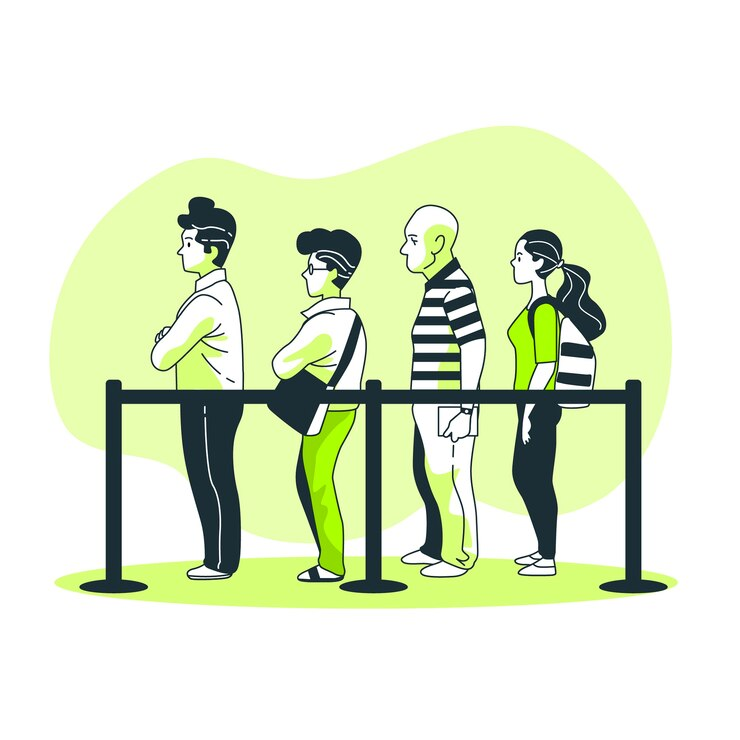
\includegraphics[width=1.2\columnwidth]
			{fig-queuePeople.jpg}
%			{example-image}
		\end{column}
		\begin{column}{.6\linewidth}
			\vspace{4cm}
			\hCite{
				\href	
					{https://www.freepik.com}
					{By Freepik}
			}
		\end{column}
		\end{columns}

	\end{column}
	\end{columns}
\end{frame}
% ~~~~~~~~~~~~~~~~~~~~~~~~~~~~~~~~~~~~~~~ A




% ~~~~~~~~~~~~~~~~~~~~~~~~~~~~~~~~~~~~~~ V
\hSection{Motivation}{}{}
% ~~~~~~~~~~~~~~~~~~~~~~~~~~~~~~~~~~~~~~ A




% ~~~~~~~~~~~~~~~~~~~~~~~~~~~~~~~~~~~~~~ V
\begin{frame}\frametitle{Motivation}

How does 

	\begin{itemize}

		\item 
		Operating Systems
		\begin{itemize}
			
			\item 
			printer keep track of files to be printed: print queue
			
			\item 
			programs run: run queue
			
		\end{itemize}
		
		\item 
		Programming
		\begin{itemize}
			
			\item 
			one model clients having service: bank queue
			
		\end{itemize}
	\end{itemize}
\end{frame}
% ~~~~~~~~~~~~~~~~~~~~~~~~~~~~~~~~~~~~~~ A




% ~~~~~~~~~~~~~~~~~~~~~~~~~~~~~~~~~~~~~~ V
\hSection{Case: Printing}{}{}
% ~~~~~~~~~~~~~~~~~~~~~~~~~~~~~~~~~~~~~~ A




% ~~~~~~~~~~~~~~~~~~~~~~~~~~~~~~~~~~~~~~ V
\begin{frame}\frametitle{Case: Printing}
	\begin{tabular}{l l l}

		% ~~~~~~~~~~~~~~~~~
		\textbf{Sent}
		&\textbf{Printing}
		&\textbf{Waiting}\\
		
		% ~~~~~~~~~~~~~~~~~
		\pause
		~
		&~
		&\begin{tikzpicture}
			\hQueue{0}{8}{0}{0}{, , , , , , , } [.5][.5]
		\end{tikzpicture}
		{\tiny noting is  printing}\\
		
		% ~~~~~~~~~~~~~~~~~
		\pause
		{\footnotesize D1}
		&{\footnotesize D1}
		&\begin{tikzpicture}
			\hQueue{0}{8}{1}{2}{D1, , , , , , , } [.5][.5]
		\end{tikzpicture}
		{\tiny D1 is sent and starts printing}\\
		
		% ~~~~~~~~~~~~~~~~~
		\pause
		{\footnotesize D2}
		&{\footnotesize D1}
		&\begin{tikzpicture}
			\hQueue{0}{8}{1}{3}{D1, D2, , , , , , } [.5][.5]
		\end{tikzpicture}
		{\tiny still printing D1}\\
		
		% ~~~~~~~~~~~~~~~~~
		\pause
		{\footnotesize D3}
		&{\footnotesize D1}
		&\begin{tikzpicture}
			\hQueue{0}{8}{1}{4}{D1, D2, D3, , , , , } [.5][.5]
		\end{tikzpicture}
		{\tiny still printing D1}\\
		
		% ~~~~~~~~~~~~~~~~~
		\pause
		~
		&{\footnotesize D2}
		&\begin{tikzpicture}
			\hQueue{0}{8}{2}{4}{D1, D2, D3, , , , , } [.5][.5]
		\end{tikzpicture}
		{\tiny D1 is done}\\
		
		% ~~~~~~~~~~~~~~~~~
		\pause
		{\footnotesize D4}
		&{\footnotesize D2}
		&\begin{tikzpicture}
			\hQueue{0}{8}{2}{5}{D1, D2, D3, D4, , , , } [.5][.5]
		\end{tikzpicture}
		{\tiny still printing D2}\\
		
		% ~~~~~~~~~~~~~~~~~
		\pause
		~
		&{\footnotesize D3}
		&\begin{tikzpicture}
			\hQueue{0}{8}{3}{5}{D1, D2, D3, D4, , , , } [.5][.5]
		\end{tikzpicture}
		{\tiny D2 is done}\\
		
		% ~~~~~~~~~~~~~~~~~
		\pause
		~
		&{\footnotesize D4}
		&\begin{tikzpicture}
			\hQueue{0}{8}{4}{5}{D1, D2, D3, D4, , , , } [.5][.5]
		\end{tikzpicture}
		{\tiny D3 is done}\\
		
		% ~~~~~~~~~~~~~~~~~
		\pause
		~
		&~
		&\begin{tikzpicture}
			\hQueue{0}{8}{5}{5}{D1, D2, D3, D4, , , , } [.5][.5]
		\end{tikzpicture}
		{\tiny D4 is done, printer idle}\\

	\end{tabular}
\end{frame}
% ~~~~~~~~~~~~~~~~~~~~~~~~~~~~~~~~~~~~~~ A




% ~~~~~~~~~~~~~~~~~~~~~~~~~~~~~~~~~~~~~~ V
\hSection{Implementation}{}{}
% ~~~~~~~~~~~~~~~~~~~~~~~~~~~~~~~~~~~~~~ A




% ~~~~~~~~~~~~~~~~~~~~~~~~~~~~~~~~~~~~~~ V
\begin{frame}\frametitle{Observations}
	\begin{columns}[T] % >>>>
	\begin{column}{.5\linewidth} % ++++ V
		\begin{itemize}
			\item
			\hEmph{Insertion}(item)
				\begin{itemize}
					\item
					on the right
					\item 
					at  \hEmph{nextAvailableLocation}\\
%					nextToLastUsedLocation
				\end{itemize}			

			\item
			\hEmph{Deletion}()
				\begin{itemize}
					\item
					on the left
					\item 
					at  \hEmph{firstUsedLocation}
				\end{itemize}			

			\item
			\hEmph{isEmpty}()
				\begin{itemize}
					\item
					\texttt{true}, if no item in it
					\item 
					\texttt{false}, otherwise
				\end{itemize}			
		\end{itemize}
	\end{column} % ++++ A
	\begin{column}{.5\linewidth} % ++++ V
%\begin{center}
\begingroup
\setlength{\tabcolsep}{3pt}
\renewcommand{\arraystretch}{.3}
	\begin{tabular}{l l l l l}
	
		% ~~~~~~~~~~~~~~~~~
		\textbf{\#} &\textbf{h} &\textbf{t}
		&\textbf{~}
		&~\\
	
		% ~~~~~~~~~~~~~~~~~
		{\scriptsize \hEmph{0}} 
		&{\scriptsize \hEmph{0}} 
		&{\scriptsize \hEmph{0}} 
		&\begin{tikzpicture}
			\hQueue{0}{5}{0}{0}{ , , , , } [.5][.5]
		\end{tikzpicture}
		&{\tiny empty}\\
	
		% ~~~~~~~~~~~~~~~~~
		{\scriptsize \hEmph{1}} 
		&{\scriptsize 0} 
		&{\scriptsize \hEmph{1}} 
		&\begin{tikzpicture}
			\hQueue{0}{5}{0}{1}{ A, , , , } [.5][.5]
		\end{tikzpicture}
		&{\tiny insert A}\\
	
		% ~~~~~~~~~~~~~~~~~
		{\scriptsize \hEmph{2}} 
		&{\scriptsize 0} 
		&{\scriptsize \hEmph{2}} 
		&\begin{tikzpicture}
			\hQueue{0}{5}{0}{2}{ A, B, , , } [.5][.5]
		\end{tikzpicture}
		&{\tiny insert B}\\
	
		% ~~~~~~~~~~~~~~~~~
		{\scriptsize \hEmph{3}} 
		&{\scriptsize 0} 
		&{\scriptsize \hEmph{3}} 
		&\begin{tikzpicture}
			\hQueue{0}{5}{0}{3}{ A, B, C, , } [.5][.5]
		\end{tikzpicture}
		&{\tiny insert C}\\
	
		% ~~~~~~~~~~~~~~~~~
		{\scriptsize \hEmph{2}} 
		&{\scriptsize \hEmph{1}} 
		&{\scriptsize 3} 
		&\begin{tikzpicture}
			\hQueue{0}{5}{1}{3}{ , B, C, , } [.5][.5]
		\end{tikzpicture}
		&{\tiny delete A}\\
	
		% ~~~~~~~~~~~~~~~~~
		{\scriptsize \hEmph{1}} 
		&{\scriptsize \hEmph{2}} 
		&{\scriptsize 3} 
		&\begin{tikzpicture}
			\hQueue{0}{5}{2}{3}{ , , C, , } [.5][.5]
		\end{tikzpicture}
		&{\tiny delete B}\\
	
		% ~~~~~~~~~~~~~~~~~
		{\scriptsize \hEmph{0}} 
		&{\scriptsize \hEmph{3}} 
		&{\scriptsize \hEmph{3}} 
		&\begin{tikzpicture}
			\hQueue{0}{5}{3}{3}{ , , , , } [.5][.5]
		\end{tikzpicture}
		&{\tiny delete C, empty}\\
	
	\end{tabular}
\endgroup
%\end{center}
	\end{column} % ++++ A
	\end{columns} % <<<<
\end{frame}
% ~~~~~~~~~~~~~~~~~~~~~~~~~~~~~~~~~~~~~~ A




% ~~~~~~~~~~~~~~~~~~~~~~~~~~~~~~~~~~~~~~ V
\begin{frame}\frametitle{Implementation with array}
	\begin{columns}[T] % >>>>
	\begin{column}{.53\linewidth} % ++++ V
		\begin{itemize}
			\item
			\hEmph{enqueue} \sout{Insertion}(item)
				\begin{itemize}
					\item
					on the right
					\item 
					at  \hEmph{tail} \sout{nextAvailableLocation}\\
%					nextToLastUsedLocation
				\end{itemize}			

			\item
			\hEmph{dequeue} \sout{Deletion}()
				\begin{itemize}
					\item
					on the left
					\item 
					at  \hEmph{head} \sout{firstUsedLocation}
				\end{itemize}			

			\item
			\hEmph{isEmpty}()
				\begin{itemize}
					\item
					\texttt{true}, if no item in it
					\item 
					\texttt{false}, otherwise
				\end{itemize}			
		\end{itemize}
		\hCite{%
			\cite{cormen2022introduction},%
			\cite{aho1974design},%
			\cite{horowitz1982fundamentals},%
			\cite{horstmann2016big}
			\cite{TheJavaTutorials}
		}

	\end{column} % ++++ A
	\begin{column}{.5\linewidth} % ++++ V
%\begin{center}
\begingroup
\setlength{\tabcolsep}{3pt}
\renewcommand{\arraystretch}{.3}
	\begin{tabular}{l l l l l}
	
		% ~~~~~~~~~~~~~~~~~
		\textbf{\#} &\textbf{h} &\textbf{t}
		&\textbf{Array}
		&~\\
	
		% ~~~~~~~~~~~~~~~~~
		{\scriptsize \hEmph{0}} 
		&{\scriptsize \hEmph{0}} 
		&{\scriptsize \hEmph{0}} 
		&\begin{tikzpicture}
			\hQueue{0}{5}{0}{0}{ , , , , } [.5][.5]
		\end{tikzpicture}
		&{\tiny empty}\\
	
		% ~~~~~~~~~~~~~~~~~
		{\scriptsize \hEmph{1}} 
		&{\scriptsize 0} 
		&{\scriptsize \hEmph{1}} 
		&\begin{tikzpicture}
			\hQueue{0}{5}{0}{1}{ A, , , , } [.5][.5]
		\end{tikzpicture}
		&{\tiny insert A}\\
	
		% ~~~~~~~~~~~~~~~~~
		{\scriptsize \hEmph{2}} 
		&{\scriptsize 0} 
		&{\scriptsize \hEmph{2}} 
		&\begin{tikzpicture}
			\hQueue{0}{5}{0}{2}{ A, B, , , } [.5][.5]
		\end{tikzpicture}
		&{\tiny insert B}\\
	
		% ~~~~~~~~~~~~~~~~~
		{\scriptsize \hEmph{3}} 
		&{\scriptsize 0} 
		&{\scriptsize \hEmph{3}} 
		&\begin{tikzpicture}
			\hQueue{0}{5}{0}{3}{ A, B, C, , } [.5][.5]
		\end{tikzpicture}
		&{\tiny insert C}\\
	
		% ~~~~~~~~~~~~~~~~~
		{\scriptsize \hEmph{2}} 
		&{\scriptsize \hEmph{1}} 
		&{\scriptsize 3} 
		&\begin{tikzpicture}
			\hQueue{0}{5}{1}{3}{ , B, C, , } [.5][.5]
		\end{tikzpicture}
		&{\tiny delete A}\\
	
		% ~~~~~~~~~~~~~~~~~
		{\scriptsize \hEmph{1}} 
		&{\scriptsize \hEmph{2}} 
		&{\scriptsize 3} 
		&\begin{tikzpicture}
			\hQueue{0}{5}{2}{3}{ , , C, , } [.5][.5]
		\end{tikzpicture}
		&{\tiny delete B}\\
	
		% ~~~~~~~~~~~~~~~~~
		{\scriptsize \hEmph{0}} 
		&{\scriptsize \hEmph{3}} 
		&{\scriptsize \hEmph{3}} 
		&\begin{tikzpicture}
			\hQueue{0}{5}{3}{3}{ , , , , } [.5][.5]
		\end{tikzpicture}
		&{\tiny delete C, empty}\\
	
	\end{tabular}
\endgroup
%\end{center}
	\end{column} % ++++ A
	\end{columns} % <<<<
\end{frame}
% ~~~~~~~~~~~~~~~~~~~~~~~~~~~~~~~~~~~~~~ A




%% ~~~~~~~~~~~~~~~~~~~~~~~~~~~~~~~~~~~~~~ V
%\begin{frame}\frametitle{Implementation with array}
%	\begin{columns}[T] % >>>>
%	\begin{column}{.5\linewidth} % ++++ V
%		\begin{itemize}
%			\item
%			Use array
%				\begin{itemize}
%					\item 
%					keep track of  \hEmph{top} 
%					\sout{lastUsedLocation} 
%				\end{itemize}			
%			\item
%			\hEmph{push}(item) \sout{insert(item)}
%				\begin{itemize}
%					\item 
%					at  \hEmph{top + 1}
%					\sout{lastUsedLocation + 1}
%				\end{itemize}			
%
%			\item
%			\hEmph{pop()} \sout{delete(item)}
%				\begin{itemize}
%					\item 
%					at \hEmph{top}
%					\sout{lastUsedLocation}
%				\end{itemize}			
%		\end{itemize}
%%		\includegraphics[width=.4\columnwidth]
%%			{fig-stack-push.pdf}
%%		\quad
%%		\includegraphics[width=.4\columnwidth]
%%			{fig-stack-pop.pdf}
%%		\\
%%		\vspace{0.2cm}	
%%		\includegraphics[width=.4\columnwidth]
%%			{fig-stack-empty.pdf}			
%		\hCite{%
%			source: CLRS~\cite{cormen2022introduction}
%		}
%		
%		\hCite{%
%			\cite{cormen2022introduction},%
%			\cite{aho1974design},%
%			\cite{horowitz1982fundamentals},%
%			\cite{horstmann2016big}
%			\cite{TheJavaTutorials}
%		}
%			
%%		\hCite{%
%%			CLRS~\cite{cormen2022introduction},%
%%			The design and analysis of computer algorithms~\cite{aho1974design},%
%%			Fundamentals of data structures~\cite{horowitz1982fundamentals},%
%%			TheJavaTutorials~\cite{TheJavaTutorials}
%%		}
%		
%	\end{column} % ++++ A
%	\begin{column}{.5\linewidth} % ++++ V
%	    	\textbf{Array}
%
%		\vspace{-0.1cm}	
%		\begin{tikzpicture}
%			\hStack{1}{4}{1}{P1}[0.5][0.5]
%		\end{tikzpicture}
%
%		\vspace{-0.1cm}	
%		\begin{tikzpicture}
%			\hStack{1}{4}{2}{P1, P2}[0.5][0.5]
%		\end{tikzpicture}
%
%		\vspace{-0.1cm}	
%		\begin{tikzpicture}
%			\hStack{1}{4}{3}{P1, P2, P3}[0.5][0.5]
%		\end{tikzpicture}
%
%		\vspace{-0.1cm}	
%		\begin{tikzpicture}
%			\hStack{1}{4}{2}{P1, P2, P3}[0.5][0.5]
%		\end{tikzpicture}
%
%		\vspace{-0.1cm}	
%		\begin{tikzpicture}
%			\hStack{1}{4}{1}{P1, P2, P3}[0.5][0.5]
%		\end{tikzpicture}
%
%		\vspace{-0.1cm}	
%		\begin{tikzpicture}
%			\hStack{1}{4}{2}{P1, P4, P3}[0.5][0.5]
%		\end{tikzpicture}
%
%		\vspace{-0.1cm}	
%		\begin{tikzpicture}
%			\hStack{1}{4}{3}{P1, P4, P5}[0.5][0.5]
%		\end{tikzpicture}
%
%		\vspace{-0.1cm}	
%		\begin{tikzpicture}
%			\hStack{1}{4}{4}{P1, P4, P5, P6}[0.5][0.5]
%		\end{tikzpicture}
%
%		\vspace{-0.1cm}	
%		\begin{tikzpicture}
%			\hStack{1}{4}{3}{P1, P4, P5, P6}[0.5][0.5]
%		\end{tikzpicture}
%
%		\vspace{-0.1cm}	
%		\begin{tikzpicture}
%			\hStack{1}{4}{2}{P1, P4, P5, P6}[0.5][0.5]
%		\end{tikzpicture}
%	\end{column} % ++++ A
%	\end{columns} % <<<<
%\end{frame}
%% ~~~~~~~~~~~~~~~~~~~~~~~~~~~~~~~~~~~~~~ A




% ~~~~~~~~~~~~~~~~~~~~~~~~~~~~~~~~~~~~~~ V
\hSection{Abstraction}{Abstract Data Types (ADT)}{}
% ~~~~~~~~~~~~~~~~~~~~~~~~~~~~~~~~~~~~~~ A




% ~~~~~~~~~~~~~~~~~~~~~~~~~~~~~~~~~~~~~~ V
\hSubsection{Abstraction-ADT}{Container}{}
% ~~~~~~~~~~~~~~~~~~~~~~~~~~~~~~~~~~~~~~ A




% ~~~~~~~~~~~~~~~~~~~~~~~~~~~~~~~~~~~~~~ V
\begin{frame}\frametitle{Abstraction-ADT: \hEmph{Container}}
	\begin{columns}[T] % >>>>
	\begin{column}{.5\linewidth} % ++++ V
	    	Container: contains items
		\begin{itemize}
			\item \hEmph{insert}(item)
			\item \hEmph{delete}(item)
			\item \hEmph{isIn}(item)
			\item \hEmph{isEmpty}()
			\item \hEmph{isFull}()
			\item \hEmph{size}()			
		\end{itemize}
	\end{column} % ++++ A
	\begin{column}{.5\linewidth} % ++++ V
		\begin{itemize}

			\item
			Insertion
			\begin{itemize}
				\item
				Order of is \hEmph{not} important
	
				\item
				Duplication is allowed
			\end{itemize}

			\item
			Deletion
			\begin{itemize}
				\item
				Any item can be deleted
			\end{itemize}
		\end{itemize}
	\end{column} % ++++ A
	\end{columns} % <<<<
\end{frame}
% ~~~~~~~~~~~~~~~~~~~~~~~~~~~~~~~~~~~~~~ A




% ~~~~~~~~~~~~~~~~~~~~~~~~~~~~~~~~~~~~~~ V
\hSubsection{Abstraction-ADT}{Set}{}
% ~~~~~~~~~~~~~~~~~~~~~~~~~~~~~~~~~~~~~~ A




% ~~~~~~~~~~~~~~~~~~~~~~~~~~~~~~~~~~~~~~ V
\begin{frame}\frametitle{Abstraction-ADT: \hEmph{Set}}
	\begin{columns}[T] % >>>>
	\begin{column}{.5\linewidth} % ++++ V
	    	Container: contains items
		\begin{itemize}
			\item insert(item)
			\item delete(item)
			\item isIn(item)
			\item isEmpty()
			\item isFull()
			\item size()			
		\end{itemize}
	\end{column} % ++++ A
	\begin{column}{.5\linewidth} % ++++ V
		\begin{itemize}

			\item
			Insertion
			\begin{itemize}
				\item
				Order of is \hEmph{not} important
	
				\item
				Duplication is  \hEmph{not} allowed
			\end{itemize}

			\item
			Deletion
			\begin{itemize}
				\item
				Any item can be deleted
			\end{itemize}
		\end{itemize}
	\end{column} % ++++ A
	\end{columns} % <<<<
\end{frame}
% ~~~~~~~~~~~~~~~~~~~~~~~~~~~~~~~~~~~~~~ A




% ~~~~~~~~~~~~~~~~~~~~~~~~~~~~~~~~~~~~~~ V
\hSubsection{Abstraction-ADT}{Stack}{}
% ~~~~~~~~~~~~~~~~~~~~~~~~~~~~~~~~~~~~~~ A




% ~~~~~~~~~~~~~~~~~~~~~~~~~~~~~~~~~~~~~~ V
\begin{frame}\frametitle{Abstraction-ADT: \hEmph{Stack}}
	\begin{columns}[T] % >>>>
	\begin{column}{.5\linewidth} % ++++ V
	    	Container: contains items
		\begin{itemize}
			\item \hEmph{enqueue}(item) \sout{insert(item)}
			\item \hEmph{dequeue()} \sout{delete(item)}
			\item \sout{isIn(item)}
			\item \hEmph{isEmpty}()
			\item \hEmph{isFull}()
			\item \sout{size()}			
		\end{itemize}
	\end{column} % ++++ A
	\begin{column}{.5\linewidth} % ++++ V
		\begin{itemize}

			\item
			\hEmph{First-In-First-Out} (\hEmph{FIFO})

			\item
			Insertion
			\begin{itemize}
				\item
				Order of is \hEmph{important} 
	
				\item
				Duplication is \hEmph{allowed}
			\end{itemize}

			\item
			Deletion
			\begin{itemize}
				\item
				\sout{Any item can be deleted}
				
				\item
				Only a \hEmph{specific} item can be deleted
			\end{itemize}
		\end{itemize}
	\end{column} % ++++ A
	\end{columns} % <<<<
\end{frame}
% ~~~~~~~~~~~~~~~~~~~~~~~~~~~~~~~~~~~~~~ A




% ~~~~~~~~~~~~~~~~~~~~~~~~~~~~~~~~~~~~~~ V
\hSubsection{Abstraction-ADT}{Queue}{}
% ~~~~~~~~~~~~~~~~~~~~~~~~~~~~~~~~~~~~~~ A




% ~~~~~~~~~~~~~~~~~~~~~~~~~~~~~~~~~~~~~~ V
\begin{frame}\frametitle{Abstraction-ADT: \hEmph{Queue}}
	\begin{columns}[T] % >>>>
	\begin{column}{.5\linewidth} % ++++ V
	    	Container: contains items
		\begin{itemize}
			\item \hEmph{push}(item) \sout{insert(item)}
			\item \hEmph{pop()} \sout{delete(item)}
			\item \sout{isIn(item)}
			\item \hEmph{isEmpty}()
			\item \hEmph{isFull}()
			\item \sout{size()}			
		\end{itemize}
	\end{column} % ++++ A
	\begin{column}{.5\linewidth} % ++++ V
		\begin{itemize}

			\item
			\hEmph{Last-In-First-Out} (\hEmph{LIFO})

			\item
			Insertion
			\begin{itemize}
				\item
				Order of is \hEmph{important} 
	
				\item
				Duplication is \hEmph{allowed}
			\end{itemize}

			\item
			Deletion
			\begin{itemize}
				\item
				\sout{Any item can be deleted}
				
				\item
				Only a \hEmph{specific} item can be deleted
			\end{itemize}
		\end{itemize}
	\end{column} % ++++ A
	\end{columns} % <<<<
\end{frame}
% ~~~~~~~~~~~~~~~~~~~~~~~~~~~~~~~~~~~~~~ A




%% ~~~~~~~~~~~~~~~~~~~~~~~~~~~~~~~~~~~~~~ V
%\hSection{Applications}{}{}
%% ~~~~~~~~~~~~~~~~~~~~~~~~~~~~~~~~~~~~~~ A









% ~~~~~~~~~~~~~~~~~~~~~~~~~~~~~~~~~~~~~~ V
\begin{frame}\frametitle{Web resources}
	\begin{itemize}

		\item 
		Problem Solving with Algorithms and Data Structures using Python
		\begin{itemize}
			
			\item 
			Home~\cite{pswads}
		
			\item
			What is a Queue~\cite{pswadsQueue} 
			
		\end{itemize}

		\item 
		The Java Tutorials by Oracle
		\begin{itemize}
			
			\item 
			Home~\cite{TheJavaTutorials}
			
			\item
			Arrays~\cite{TheJavaTutorialsArray}
			
			\item
			Generics~\cite{TheJavaTutorialsGenerics}
			
		\end{itemize}
		
	\end{itemize}
\end{frame}
% ~~~~~~~~~~~~~~~~~~~~~~~~~~~~~~~~~~~~~~ A



% ~~~~~~~~~~~~~~~~~~~~~~~~~~~~~~~~~~~~~~ V References bib
\begin{frame}[allowframebreaks]\frametitle{References}
	\setbeamertemplate{bibliography item}[text] % sets numbers in references
%	\bibliographystyle{abbrv}
%	\bibliographystyle{apalike}
%	\bibliographystyle{ieeetr}
	\bibliographystyle{IEEEtran}
	%
	\tiny\bibliography{../hbcommon/bingol-DataStructures} % bib file

	
\end{frame}
% ~~~~~~~~~~~~~~~~~~~~~~~~~~~~~~~~~~~~~~ A

% ~~~~~~~~~~~~~~~~~~~~~~~~~~~~~~~~~~~~~~~ 
\end{document}
